\setlength{\parindent}{2em} %首行缩进

\section*{實驗目的:}


\section*{實驗步驟:}


\section*{實驗結果及討論:}
\subsection*{結果:}
\begin{enumerate}
  \item 根據\prettyref{fig:gel_filtration},膠體過濾實驗中 OD$_{595nm}$的峰值發生在Fraction 3,而OD$_{450nm}$的峰值發生在Fraction 6。
  \item 根據\prettyref{tab:BSA}, \prettyref{fig:stand_curve} ,得知BSA濃度標準曲線 $y=0.0673x+0.0301,\ R^2=0.966$,即可推算 Fraction 3 的濃度為 0.804 \mug/\mul。 
  \item Fraction 3 的層析液約為 350\mul ,BSA 回收率為
  $$
  \frac{0.804(\mug/\mul)\times 350(\mul)}{1(\mug/\mul)\times 500(\mul)}=0.562
  $$


\end{enumerate}


  




\subsection*{實驗數據:}

\begin{table}[h]
\begin{minipage}[t]{0.45\textwidth}
  \setlength{\abovecaptionskip}{0cm} % 调整caption间距
  \caption{膠體層析吸光值數據}\label{tab:gel_filtration}
  \begin{tabular}{lll}
    \toprule
    fraction no.&OD$_{595nm}$&OD$_{450nm}$\\
    \midrule
    1&1.695&0.241\\
    2&1.767&0.204\\
    3&2.399&0.183\\
    4&0.953&0.226\\
    5&1.284&0.673\\
    6&1.196&0.818\\
    7&1.196&0.229\\
    8&1.481&0.198\\
    \bottomrule
  \end{tabular}
\end{minipage}
\begin{minipage}[t]{0.45\textwidth}
  \setlength{\abovecaptionskip}{0cm} % 调整caption间距
  \caption{BSA吸光值數據}\label{tab:BSA}
  \begin{tabular}{lll}
    \toprule
    BSA (mg)&OD$_{595nm}$&raw data\\
    \midrule
    0&0&0.759\\
    2&0.22&0.979\\
    4&0.328&1.087\\
    6&0.364&1.123\\
    8&0.552&1.311\\
    10&0.736&1.495\\
    \midrule
    A(2\mul\ unknown)&0.116&0.875\\
    B(4\mul\ unknown)&0.291&1.050\\
    \bottomrule
  \end{tabular}
\end{minipage}
\end{table}

\begin{table}[ht]
  \setlength{\abovecaptionskip}{0cm} % 调整caption间距
  \setlength{\tabcolsep}{10mm}{
  \caption{BAS吸光值回歸直線與回收率} 
  \begin{tabular}{llll}
    \toprule
    y=a+bx&\\
    \midrule
    a&0.0673\\
    b&0.0301\\
    R$^2$&0.966\\
    \midrule
    A濃度&0.638 \mug/\mul\\
    B濃度&0.969 \mug/\mul\\
    平均濃度&0.804 \mug/\mul\\
    回收率&0.562\\
    \bottomrule
  \end{tabular}}
\end{table}

\subsection*{實驗作圖:}

\begin{figure}[H]
\centering
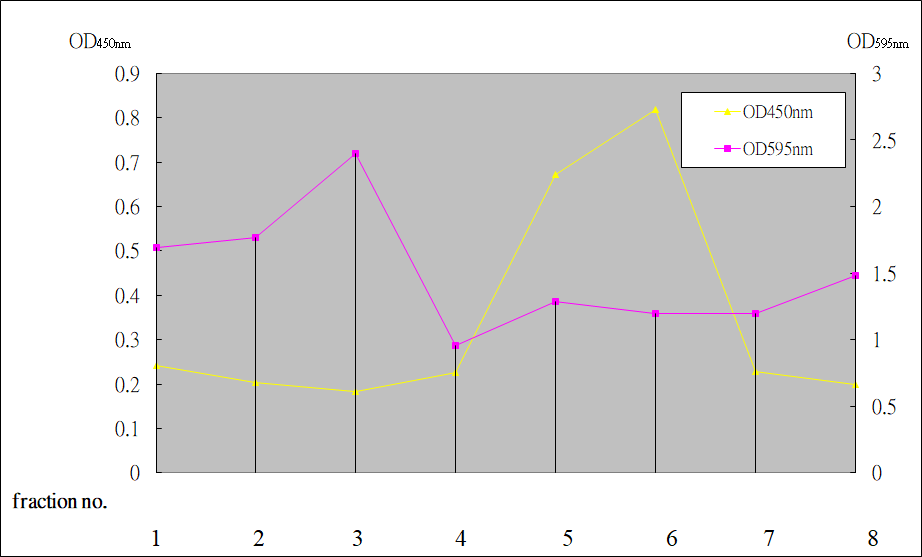
\includegraphics[width=.8\textwidth]{paste_src/2023-10-18-22-15-33.png}
\caption{膠體層析吸光值}
\label{fig:gel_filtration}
\vspace{1em}
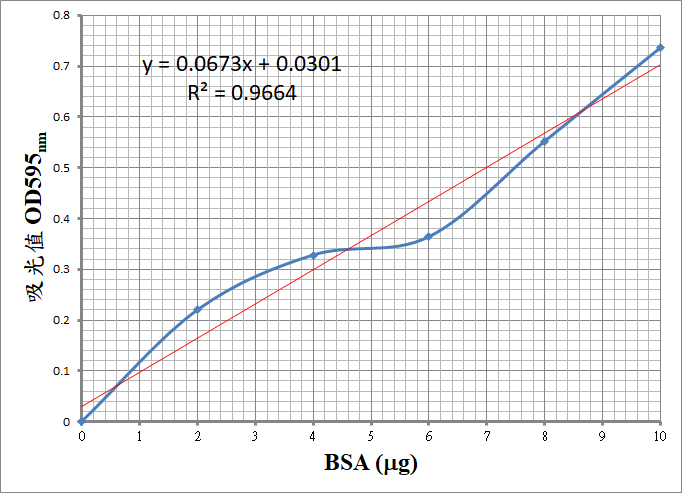
\includegraphics[width=.8\textwidth]{paste_src/2023-10-18-22-23-08.png}
\caption{BSA吸光值標準曲線}
\label{fig:stand_curve}
\end{figure}




\subsection*{實驗討論:}


\bibliography{bibfile} 
\bibliographystyle{unsrt}
